\section{Grafo dirigido}\label{DirectedGraph}
Un grafo \( G(V,E) \) es una colección de puntos, llamados vértices o nodos \( V = \{ v_1, v_2, \dots \} \), y segmentos de línea que conectan esos puntos, llamados aristas o arcos (en inglés \textit{edges}) \( E = \{ e_1, e_2, \dots \} \); cada arista \( e \) tiene dos \textit{\gls{endpoints}}, que son vértices.

Un digrafo o grafo dirigido \( G(V,E) \) se define de manera similar a un grafo, excepto que el par de \textit{\gls{endpoints}} \( (u, v) \) de cada arista ahora está ordenado. Se escribe \( u \xrightarrow{\text{e}} v \), dónde \( u \) es el vértice inicial de \( e \); y \( v \) es el vértice final de \( e \). Se dice que la arista \( e \) está dirigida de \( u \) a \( v \) \cite{book:even2011graph}.

\begin{figure}[H]
	\centering
	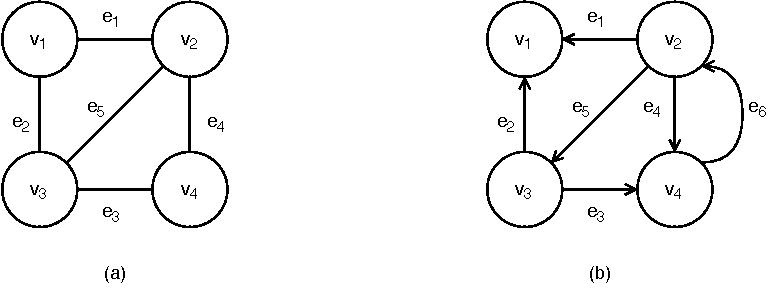
\includegraphics[width=0.8\linewidth]{doc/DirectedGraph/img/directed-undirected-graph}
	\caption{Tipos de grafos. (a) No dirigido. (b) Dirigido o digrafo. }
	\label{fig:directed-undirected-graph}
\end{figure}